\begin{frame}
    \frametitle{Signaalverwerking}
    
    \begin{figure}
        \centering
        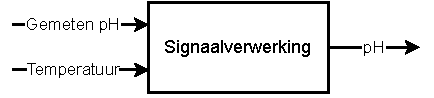
\includegraphics[width=\textwidth]{signaalverwerkingBlokje}
    \end{figure}

\end{frame}

\begin{frame}
    \frametitle{Signaalverwerking}
    
    \begin{figure}
        \centering
        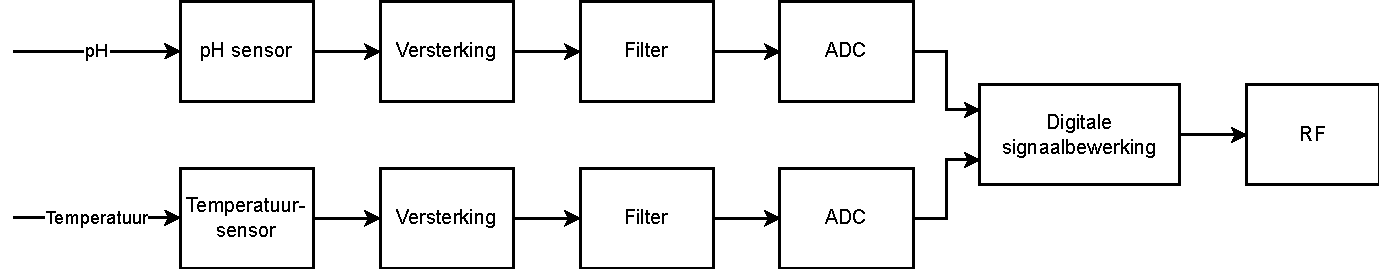
\includegraphics[width=\textwidth]{analogeBewerkingsFunctie.pdf}
    \end{figure}

\end{frame}

\begin{frame}
    \frametitle{Energie budget}
    \begin{table}[ht]
        \centering
        \begin{tabular}{l|l}
            Func. blok          & Vermogen [mW] \\
            \hline                              
            Reken $U_{GS}\rightarrow$pH & 0.6   \\
            ADC                 & 1             \\
            AA-filter           & 0.2           \\
            Meet $U_{GS}$       & 0.2           \\
            Zenden              & 5             \\
            Oplader             & 0.5           \\
            Beveiliging         & 0.5           \\
            Spanningsregeling   & 1             \\ 
            \hline
            \hline
            Totaal              & 9
            
        \end{tabular}
        \label{tab:energieBudgetEstimatie}
    \end{table}
    
    Waardes zijn boven de berekend theoretisch minimum
\end{frame}